\documentclass{article}
\usepackage[a4paper, left=2cm, right=2cm, top=3cm, bottom=3cm, headheight=35pt, includehead]{geometry}

\usepackage[english]{babel}
\usepackage[utf8]{inputenc}
\usepackage{fancyhdr}

\usepackage{enumitem}
\usepackage{amsmath}
\usepackage{mathtools}
\usepackage{listings}


\lstset{mathescape=true,
		morekeywords={if,else,and,then,for,return}}

\pagestyle{fancy}
\fancyhf{}
\lhead{\today \\ Andrés Montoya, 405409 \\ Laura Koch, 406310 }
\chead{Introduction to Artificial Intelligence \\ Assignment 01}
\rhead{ Lennart Holzenkamp, 407761 \\ Simon Michau, 406133 \\ Til Mohr, 405959}

\begin{document}

\section*{Exercise 1.1}
\begin{enumerate}[label=(\alph*)]
	\item	Yes, the elevator control can be regarded as an agent, as it follows the architecture of rational agents.

			It has sensors (buttons) to percieve (button status) the environment (elevator + floors) and will operate (move up/down + open/close doors) based on that input, with the goal of transporting people.

			The elevator control agent is reflexive with an internal state, as it always remembers the current floor the elevator is in.

			Depending on the implementation of $\phi_v^u$ the agent may be goal-based or utility-based. If $\phi_v^u$ simply selects a random floor to be served next, it is just goal-based. If $\phi_v^u$ selects the next floor to be served while minimizing waiting time for example, it is utility-based.
	\item	\begin{itemize}
				\item	Persons transported per hour
				\item	Average waiting time for buttons pressed in the elevator
				\item	Average waiting time for buttons pressed on a floor
			\end{itemize}
	\item	The following function $\phi_v^u$ operates best when M/W are implemented as a queue. \\
			First we select the nearest requested floor based on waiting time, then we check if there is any floor between that and the current floor.
\begin{lstlisting}
next $\leftarrow$ f
m $\leftarrow$ M[0]
w $\leftarrow$ W[0]

if m is null and w is null then
	return f
if m is null and w is not null then
	next $\leftarrow$ w
if m is not null and w is null then
	next $\leftarrow$ m
if m is not null and w is not null then
	if |m-f|>|w-f| then
		next $\leftarrow$ w
	else
		next $\leftarrow$ m

for x in M $\cup$ W
	if |x-f|<|next-f| then
		next $\leftarrow$ x

return x
\end{lstlisting}
\end{enumerate}

\section*{Exercise 1.2}
\begin{enumerate}[label=(\alph*)]
	\item	\begin{itemize}
				\item	semi-accessible: Information on number of people waiting on each floor and number of people inside the elevator could optimize the agent
				\item	deterministic: the elevator chooses his next action solely based on the current floor and the goal floor (assuming that $\phi^u_v$ is not random)
				\item	episodc: choice of action only depends on current state
				\item	dynamic: new buttons can be pressed while deciding
				\item	discrete: the elevators environment consists of the floors it can visit, which are discrete
			\end{itemize}
	\item	\begin{itemize}
				\item nonaccessible: many aspects of the internet are inaccessible to search engines, e.g. many databases or networks behind firewalls
				\item
				\item episodic if cookies do not affect the results of a search, nonepisodic otherwise
				\item dynamic: content on the internet can change any time, e.g. when a website is updated or put down
				\item assuming the environment of the internet consists of any type of object (like websites, databases, etc.) in it, the environment would be discrete since the individual objects are atomic
			\end{itemize}
	\item	\begin{itemize}
				\item assuming the relevant aspects for the rover are his spacial surroundings, they must be accessible to the rover in order for it to navigate the surface of mars
				\item given that there are external influences like duststorms on mars which would affect the rover, one can argue that the environment is not entirely deterministic
				\item nonepisodic: since the rover might not be supposed to go back to a place it has already visited (or the contrary) the previous positions/states determine the current actions
				\item dynamic: the environment can change, for example when rocks roll down a hill or a sandstorm occurs
				\item continuous: since a rover is a mobile robot performing in the real world it obviously operates in a continuous environment (as mentioned in the lecture)
			\end{itemize}
\end{enumerate}

\section*{Exercise 1.3}
\begin{enumerate}[label=(\alph*)]
	\item	Choose a random direction and suck.
	\item
	\item	Those agents don't know their initial position and do not store any information about their past actions, so they cannot backtrack to their initial position.
\end{enumerate}

\section*{Exercise 1.4}
Since the environment is fully observable, we can simple check, if the current room is dirty or not. If it is dirty, we clean it, then switch rooms and repeat the cleaning step.\\
Since we never suck when the room is clean, we cannot make it dirty with a probability of 10\%.\\
State sequences:
\begin{itemize}
	\item	$1 \rightarrow 5 \rightarrow 6 \rightarrow 8$
	\item	$2 \rightarrow 4 \rightarrow 3 \rightarrow 7$
	\item	$3 \rightarrow 7$
	\item	$4 \rightarrow 3 \rightarrow 7$
	\item	$5 \rightarrow 6 \rightarrow 8$
	\item	$6 \rightarrow 8$
	\item	$7$
	\item	$8$
\end{itemize}

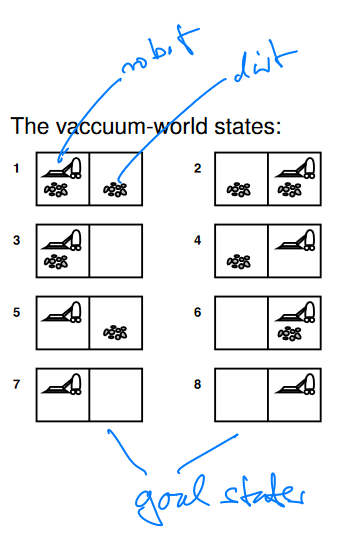
\includegraphics{1.4.png}

\end{document}